%************************************************
\section*{Methodology}\label{ch:methodology}
%************************************************

\subsection*{Research Questions}\label{sec:research_questions}

\textbf{RQ1: What are the characteristics of structural commit-feature interactions?}

We intend to research two main properties that will already give a lot of insight into the development process of features and usage of commits.
Firstly, we will examine the statistical distribution of how many commits, features interact with structurally.
This will directly give a rough estimation on how many commits were needed to create a feature.
Secondly, we want to examine how many features a commit affects structurally, e.g. how many features a commit usually changes. 
This is especially interesting when considering best practices surrounding the usage of commits.

\begin{center}
\begin{tabular}{cc}
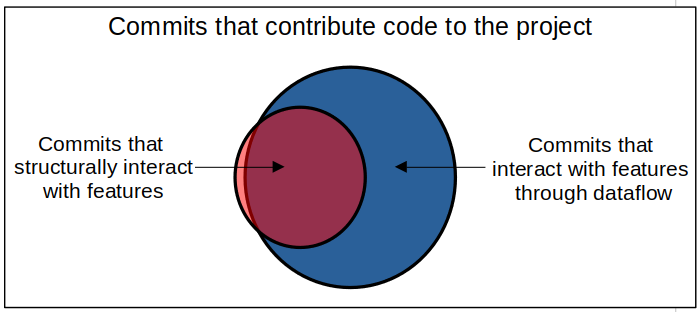
\includegraphics[height=6cm]{gfx/Commits-of-a-Software-Project.png}
\end{tabular}
\captionof{figure}{Kinds of Commits in a Software Project investigated in this work}
\end{center}

It is preferred to keep commits granular meaning they should only fix a single bug or, in our case, change a single feature.
Acquiring data on this issue will show how strictly this policy is enforced in software development. \\

\textbf{RQ2: How do commits interact with features through dataflow?}

Previous research has focused solely on dataflow interactions between commits.
We have already discussed the importance of research in the area and why further research is necessary.
That's why we want to provide first insights on the properties of dataflow-based commit-feature interactions.
One could form several assumptions about them based on a basic understanding of commits and features in software engineering.
Showing wether these can be based on statiscal evidence will either secure or change the way we view them.
Specifically, we want to investigate how interconnected commits and features are by analyzing the amount of features a commit usually affects through dataflow.
Showing what fraction of all commits contributing code to a project affect data of a feature will provide further insight on this. 
Since it's plausible that commits constituting code of a feature might be more likely to influence the data used in said feature, we want to differentiate between these types of commits here.
This can be accomplished with the help of our structural commit-feature interaction analysis. 
This will give us important information on how likely commits, that aren't part of feature, are to influence the data of a feature. \\

\textbf{RQ3: How do authors implement features?}

Usually there are many programmers working on the same software project, implementing different features, sometimes alone, sometimes with the help of colleagues.
We want to shine some light on the exact statistics of this by using structural commit-feature interactions and high-level repository information.
One major question is how many authors implement a feature on average, where considering feature-size could help put this data into perspective.
%Digging deeper, we aim to gauge the amount of code each developer of a feature contributes. 
%This way we can find out the extend to which the contribution varies between programmers.
The collected results could serve as advice for software companies on how to balance workload on to-be implemented features. 

\subsection*{Operationalization}\label{sec:operationalization}

The detection of structural as well as dataflow-based commit-feature interactions is implemented in VaRA \cite{VaRA2023}.
VaRA offers two main functionalities for this. 
The first one is the detection of feature- and commit-code, which is accomplished by being able to receive all commits and features an llvm-IR instruction belongs to.
Thus we can collect all structural commit-feature interactions by iterating over all instructions in the code space.
Inside an instruction we save every combination of commits and features as a CFI.
It follows that, in order for an instruction to have a single interaction, it needs to be part of at least one commit as well as one feature.
For each structural CFI we also save the amount of instructions said cfi occurs in. 
This is accomplished by incrementing the instruction counter if we happen to encounter a duplicate CFI. 
VaRA is also able to track taints of values along program flow, where taints essentially carry information on which commits have previously affected that specific value.
Similarly to structural interactions, dataflow-based commit-feature interactions are iteratively collected on instruction level.
In this case we speak of an dataflow interaction when an instruction both has a commit taint and belongs to a feature.
Consequently this instruction uses a value that was changed by a commit earlier in the program while stemming from code constituting a feature.
For our research we will examine numerous software projects to get a wide range of reference data, as commit-feature interactions could potentially vary greatly between different code spaces.
Accordingly, the VaRA-Tool-Suite was extended making it possible to generate a report comprising all found CFIs of an according type in a software project.
This will aid us in examining several software projects to gain sufficient and sensible data about commit-feature interactions.
The created reports will also be evaluated in the VaRA-Tool-Suite, which offers support to process and display statstics of the generated data. \\

\textbf{RQ1: What are the characteristics of structural commit-feature interactions?}

The needed data will be collected by creating the aforementioned reports comprimising all structural commit-feature interactions of a chosen software project.
The collected data is then evaluated by iterating over all found commit-feature interactions.
For each encountered feature we save the commits it interacts with and add up the amount of instructions where a structural interaction with said feature occurs.
We have previously noted that a feature only structurally interacts with a commit that has contributed code to said feature.
Besides that each line of code in a git project was added or changed by a commit, which means that each line of code belonging to a feature also belongs to a commit.
Therefore all the commits of a feature saved during evaluation are the commits that constitue the code space of a feature. 
With this data, it's possible to calculate the average amount of commits used to create a feature, while being able to correlate this with its size, in our case, its number of instructions.
For the evaluation of the second point, we iterate over all found structural commit-feature interactions again, but instead save the features each encountered commit interacts with. \\

\textbf{RQ2: How do commits interact with features through dataflow?}

The projects investigated for dataflow-based commit-feature interactions will be the same projects investigated for structural commit-feature interactions.
This choice will allow more insight into a single project and allow us to combine both analyses as will be discussed below.
In this RQ we consider all commits that currently contribute code to the project, which we can extract from high level repository information of the project.
For each commit we will save whether and if yes which features they interact with through dataflow.
Similarly to RQ1, this is carried out by iterating over the dataflow-based commit-feature interactions in the created reports.
The acquired information makes it possible to calculate what fraction of commits interact with features through dataflow.
For commits that do have dataflow-based interactions with features, we will examine how many features they interact with on average.
The dicussed separation for said commits into those that are part of a feature and those that aren't is accomplished with the usage of already created structural reports. 
We can find out whether a commit is part of a feature by checking if it is part of a structural commit-feature interaction in the according report. \\

\textbf{RQ3: How do authors implement features?}

For this RQ we will examine the same projects as the previous RQs.
That way we can reuse data produced in RQ1 to map each feature to the authors that implemented it.
In RQ1 we have already mapped each feature to the commits it interacts with, e.g. that contribute code to it.
It's possible to retract the authors of these commits by searching through high-level repository information with their hashes.
This will directly give us the authors that implemented a feature.
The amount of instructions that stem from code belonging to a feature has also been calculated for RQ1.
With this information we can measure the correlation between feature-size and the amount of developers needed to implement it.
%Furthermore we want to estimate the amount of code a developer contributes to a feature by equating it with the amount of instructions.

\subsection*{Expectations}\label{sec:expectations}

In this section, discuss the results you expect to get from your evaluation.

\subsection*{Threats to Validity}\label{sec:threats}

In this section, discuss the threats to internal and external validity you have to be aware of during the evaluation.
